% Options for packages loaded elsewhere
\PassOptionsToPackage{unicode}{hyperref}
\PassOptionsToPackage{hyphens}{url}
%
\documentclass[
  10pt,
  ignorenonframetext,
]{beamer}
\usepackage{pgfpages}
\setbeamertemplate{caption}[numbered]
\setbeamertemplate{caption label separator}{: }
\setbeamercolor{caption name}{fg=normal text.fg}
\beamertemplatenavigationsymbolsempty
% Prevent slide breaks in the middle of a paragraph
\widowpenalties 1 10000
\raggedbottom
\setbeamertemplate{part page}{
  \centering
  \begin{beamercolorbox}[sep=16pt,center]{part title}
    \usebeamerfont{part title}\insertpart\par
  \end{beamercolorbox}
}
\setbeamertemplate{section page}{
  \centering
  \begin{beamercolorbox}[sep=12pt,center]{part title}
    \usebeamerfont{section title}\insertsection\par
  \end{beamercolorbox}
}
\setbeamertemplate{subsection page}{
  \centering
  \begin{beamercolorbox}[sep=8pt,center]{part title}
    \usebeamerfont{subsection title}\insertsubsection\par
  \end{beamercolorbox}
}
\AtBeginPart{
  \frame{\partpage}
}
\AtBeginSection{
  \ifbibliography
  \else
    \frame{\sectionpage}
  \fi
}
\AtBeginSubsection{
  \frame{\subsectionpage}
}

\usepackage{amsmath,amssymb}
\usepackage{iftex}
\ifPDFTeX
  \usepackage[T1]{fontenc}
  \usepackage[utf8]{inputenc}
  \usepackage{textcomp} % provide euro and other symbols
\else % if luatex or xetex
  \usepackage{unicode-math}
  \defaultfontfeatures{Scale=MatchLowercase}
  \defaultfontfeatures[\rmfamily]{Ligatures=TeX,Scale=1}
\fi
\usepackage{lmodern}
\usetheme[]{Boadilla}
\ifPDFTeX\else  
    % xetex/luatex font selection
\fi
% Use upquote if available, for straight quotes in verbatim environments
\IfFileExists{upquote.sty}{\usepackage{upquote}}{}
\IfFileExists{microtype.sty}{% use microtype if available
  \usepackage[]{microtype}
  \UseMicrotypeSet[protrusion]{basicmath} % disable protrusion for tt fonts
}{}
\makeatletter
\@ifundefined{KOMAClassName}{% if non-KOMA class
  \IfFileExists{parskip.sty}{%
    \usepackage{parskip}
  }{% else
    \setlength{\parindent}{0pt}
    \setlength{\parskip}{6pt plus 2pt minus 1pt}}
}{% if KOMA class
  \KOMAoptions{parskip=half}}
\makeatother
\usepackage{xcolor}
\newif\ifbibliography
\setlength{\emergencystretch}{3em} % prevent overfull lines
\setcounter{secnumdepth}{-\maxdimen} % remove section numbering


\providecommand{\tightlist}{%
  \setlength{\itemsep}{0pt}\setlength{\parskip}{0pt}}\usepackage{longtable,booktabs,array}
\usepackage{calc} % for calculating minipage widths
\usepackage{caption}
% Make caption package work with longtable
\makeatletter
\def\fnum@table{\tablename~\thetable}
\makeatother
\usepackage{graphicx}
\makeatletter
\def\maxwidth{\ifdim\Gin@nat@width>\linewidth\linewidth\else\Gin@nat@width\fi}
\def\maxheight{\ifdim\Gin@nat@height>\textheight\textheight\else\Gin@nat@height\fi}
\makeatother
% Scale images if necessary, so that they will not overflow the page
% margins by default, and it is still possible to overwrite the defaults
% using explicit options in \includegraphics[width, height, ...]{}
\setkeys{Gin}{width=\maxwidth,height=\maxheight,keepaspectratio}
% Set default figure placement to htbp
\makeatletter
\def\fps@figure{htbp}
\makeatother
\newlength{\cslhangindent}
\setlength{\cslhangindent}{1.5em}
\newlength{\csllabelwidth}
\setlength{\csllabelwidth}{3em}
\newlength{\cslentryspacingunit} % times entry-spacing
\setlength{\cslentryspacingunit}{\parskip}
\newenvironment{CSLReferences}[2] % #1 hanging-ident, #2 entry spacing
 {% don't indent paragraphs
  \setlength{\parindent}{0pt}
  % turn on hanging indent if param 1 is 1
  \ifodd #1
  \let\oldpar\par
  \def\par{\hangindent=\cslhangindent\oldpar}
  \fi
  % set entry spacing
  \setlength{\parskip}{#2\cslentryspacingunit}
 }%
 {}
\usepackage{calc}
\newcommand{\CSLBlock}[1]{#1\hfill\break}
\newcommand{\CSLLeftMargin}[1]{\parbox[t]{\csllabelwidth}{#1}}
\newcommand{\CSLRightInline}[1]{\parbox[t]{\linewidth - \csllabelwidth}{#1}\break}
\newcommand{\CSLIndent}[1]{\hspace{\cslhangindent}#1}

\makeatletter
\makeatother
\makeatletter
\makeatother
\makeatletter
\@ifpackageloaded{caption}{}{\usepackage{caption}}
\AtBeginDocument{%
\ifdefined\contentsname
  \renewcommand*\contentsname{Table of contents}
\else
  \newcommand\contentsname{Table of contents}
\fi
\ifdefined\listfigurename
  \renewcommand*\listfigurename{List of Figures}
\else
  \newcommand\listfigurename{List of Figures}
\fi
\ifdefined\listtablename
  \renewcommand*\listtablename{List of Tables}
\else
  \newcommand\listtablename{List of Tables}
\fi
\ifdefined\figurename
  \renewcommand*\figurename{Figure}
\else
  \newcommand\figurename{Figure}
\fi
\ifdefined\tablename
  \renewcommand*\tablename{Table}
\else
  \newcommand\tablename{Table}
\fi
}
\@ifpackageloaded{float}{}{\usepackage{float}}
\floatstyle{ruled}
\@ifundefined{c@chapter}{\newfloat{codelisting}{h}{lop}}{\newfloat{codelisting}{h}{lop}[chapter]}
\floatname{codelisting}{Listing}
\newcommand*\listoflistings{\listof{codelisting}{List of Listings}}
\makeatother
\makeatletter
\@ifpackageloaded{caption}{}{\usepackage{caption}}
\@ifpackageloaded{subcaption}{}{\usepackage{subcaption}}
\makeatother
\makeatletter
\@ifpackageloaded{tcolorbox}{}{\usepackage[skins,breakable]{tcolorbox}}
\makeatother
\makeatletter
\@ifundefined{shadecolor}{\definecolor{shadecolor}{rgb}{.97, .97, .97}}
\makeatother
\makeatletter
\makeatother
\makeatletter
\makeatother
\ifLuaTeX
  \usepackage{selnolig}  % disable illegal ligatures
\fi
\IfFileExists{bookmark.sty}{\usepackage{bookmark}}{\usepackage{hyperref}}
\IfFileExists{xurl.sty}{\usepackage{xurl}}{} % add URL line breaks if available
\urlstyle{same} % disable monospaced font for URLs
\hypersetup{
  pdftitle={Introduction to Longitudinal Modified Treatment Policies},
  pdfauthor={Kat Hoffman},
  hidelinks,
  pdfcreator={LaTeX via pandoc}}

\title{Introduction to Longitudinal Modified Treatment Policies}
\subtitle{A solution for studying complex, continuous, and/or
time-varying exposures}
\author{Kat Hoffman}
\date{2024-02-15}

\begin{document}
\frame{\titlepage}
\ifdefined\Shaded\renewenvironment{Shaded}{\begin{tcolorbox}[borderline west={3pt}{0pt}{shadecolor}, enhanced, boxrule=0pt, breakable, sharp corners, interior hidden, frame hidden]}{\end{tcolorbox}}\fi

\begin{frame}{Overview}
\protect\hypertarget{overview}{}
\newcommand{\Pdist}{\mathsf{P}}
\newcommand{\dint}{\mathsf{d}}
\newcommand{\E}{\mathsf{E}}
\newcommand{\Ec}{\mathbb{E}}
\newcommand{\V}{\mathsf{Var}}
\newcommand{\M}{\mathcal{M}}
\newcommand{\1}{\mathbbm{1}}
\newcommand{\pr}{\mathsf{pr}}

\begin{itemize}
\tightlist
\item
  Discussing a tutorial paper on Longitudinal Modified Treatment
  Policies
\item
  Target audience: epidemiologists and applied statisticians
\item
  Based on methodology proposed in \emph{Díaz et al.~(2021)}
  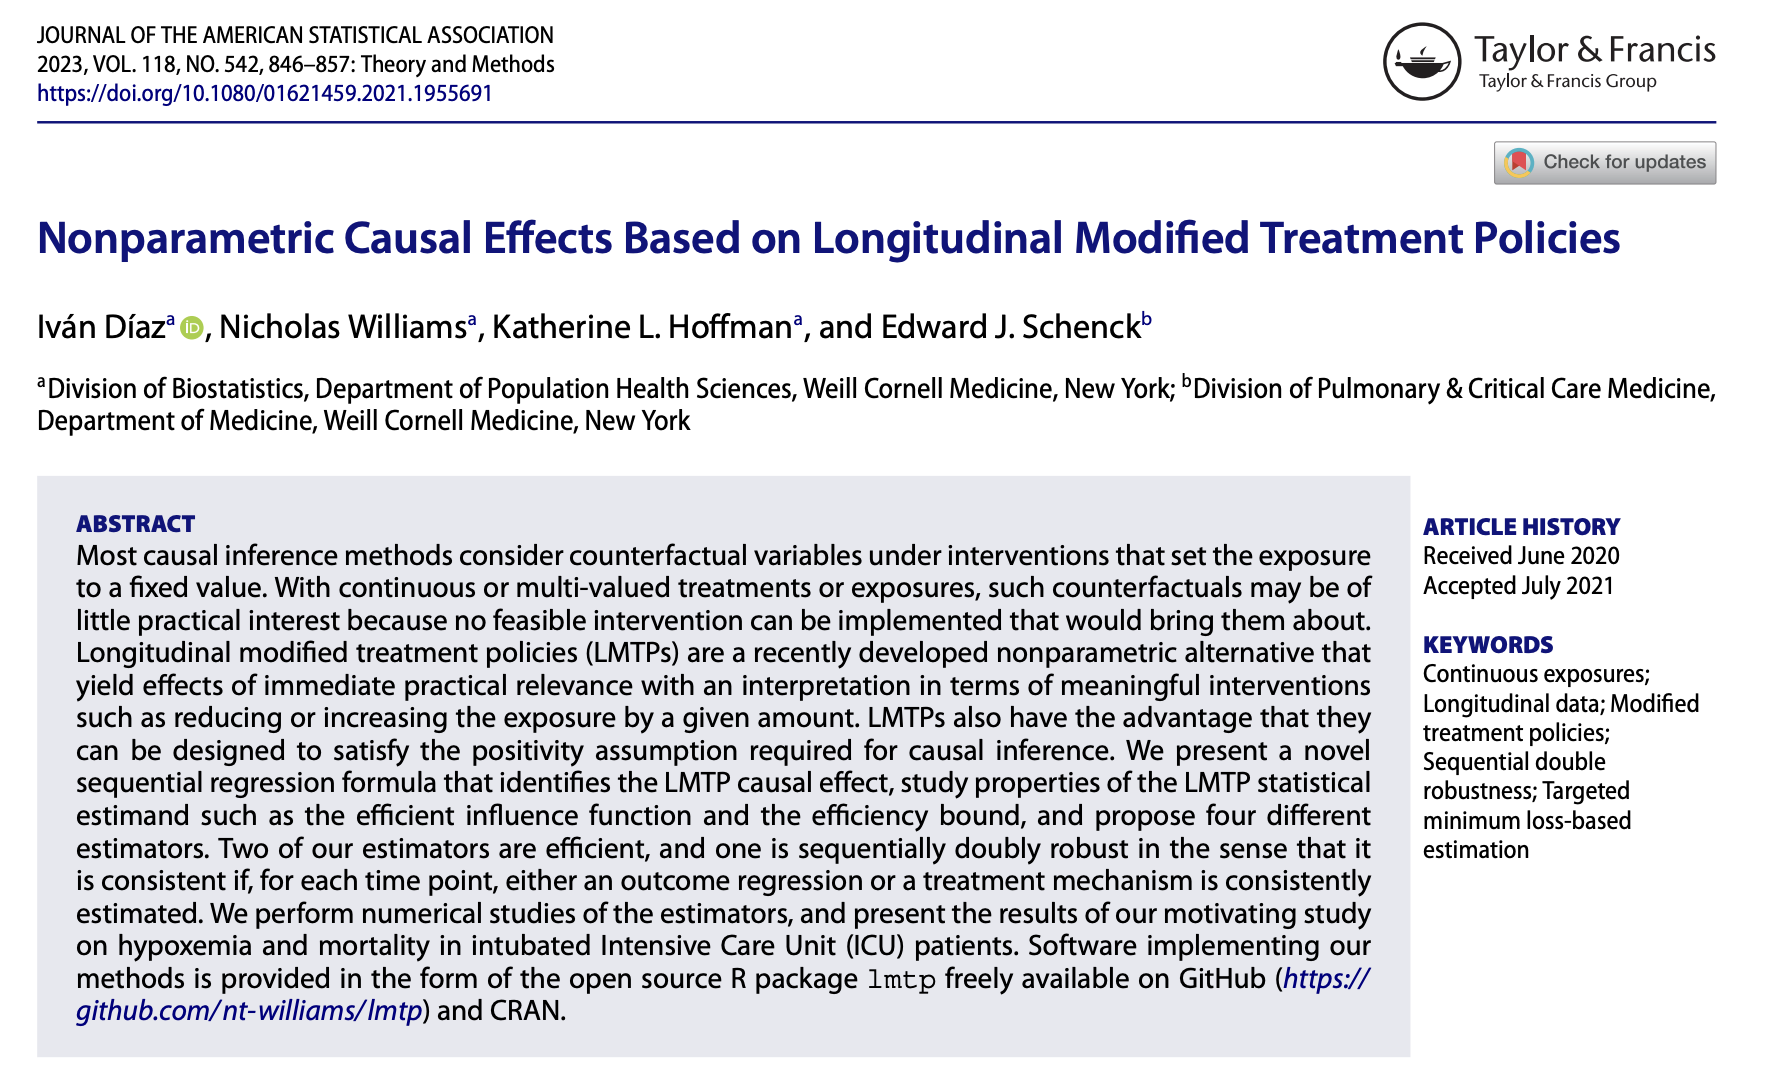
\includegraphics{img/jasa_ss.png}
\end{itemize}
\end{frame}

\begin{frame}{Methodology motivation}
\protect\hypertarget{methodology-motivation}{}
\begin{itemize}
\item
  Many causal inference methods and tutorials focus on binary exposures
  at a single time point

  \begin{itemize}
  \item
    Continuous/multi-level categorical exposures common in applied
    research, but methods, software, teaching materials are more limited
  \item
    Many studies have time-varying exposures, but methods are even less
    common

    \begin{itemize}
    \tightlist
    \item
      If there are time-dependent confounders, we require special
      methods to appropriately estimate treatment effects
    \end{itemize}
  \end{itemize}
\end{itemize}
\end{frame}

\begin{frame}{Methodology motivation}
\protect\hypertarget{methodology-motivation-1}{}
\begin{itemize}
\item
  Positivity assumption is essential to causal inference

  \begin{itemize}
  \item
    Violations are common in cases of categorical and continuous
    exposures
  \item
    Violations are exacerbated when there are multiple time points
  \end{itemize}
\item
  An active area of statistical research is defining, identifying, and
  estimating alternative causal estimands which may increase the
  likelihood of meeting the positivity assumption
\end{itemize}
\end{frame}

\begin{frame}{One solution: Longitudinal Modified Treatment Policies
(LMTPs)}
\protect\hypertarget{one-solution-longitudinal-modified-treatment-policies-lmtps}{}
\begin{itemize}
\item
  Diaz et al.~(2021) proposed longitudinal interventions which depend on
  an individual's \emph{natural value of treatment}

  \begin{itemize}
  \item
    Natural value of treatment: the value treatment would take at time
    \(t\) if an intervention was discontinued right before time \(t\)
  \item
    Provided identification result and doubly/sequentially robust
    estimation algorithms
  \end{itemize}
\item
  Methodology generalizes static, dynamic, and some stochastic
  interventions, so can accommodate:

  \begin{itemize}
  \tightlist
  \item
    binary, categorical, continuous, and multiple exposures
  \item
    binary, continuous, time-to-event outcomes, competing risks,
    informative right-censoring, clustering
  \item
    point-in-time and time-varying settings
  \end{itemize}
\item
  LMTPs help address violations of the positivity assumption, because we
  define an alternative interventions for which positivity holds by
  design
\end{itemize}
\end{frame}

\begin{frame}{Tutorial organization}
\protect\hypertarget{tutorial-organization}{}
\begin{enumerate}
\item
  Review static and dynamic interventions, and introduce (longitudinal)
  modified treatment policies
\item
  High-level theory:

  \begin{itemize}
  \tightlist
  \item
    Identification in point-in-time and time-varying settings
  \item
    Estimation procedures
  \end{itemize}
\item
  Application:

  \begin{itemize}
  \tightlist
  \item
    Provide examples of research questions that could be (or already
    have!) been addressed using LMTPs
  \item
    Illustrate application of an LMTP to estimate the effect of
    intubation timing on mortality in COVID-19 patients, using a
    real-world longitudinal observational data set
  \end{itemize}
\end{enumerate}
\end{frame}

\hypertarget{notation-and-setup}{%
\section{Notation and setup}\label{notation-and-setup}}

\begin{frame}{Notation}
\protect\hypertarget{notation}{}
\begin{itemize}
\item
  \(Z_1, ..., Z_n \overset{\text{iid}}{\sim} \mathsf{P}\)

  \begin{itemize}
  \item
    \(\mathsf{P}\) represents a longitudinal process and may contain any
    number of time points, but for simplicity we will describe a
    distribution with only two time points, \(t \in \{0,1\}\)
  \item
    For each unit in the study, we observe a set of random variables
    \(Z = (L_0, A_0, L_1, A_1, Y)\)
  \end{itemize}
\end{itemize}

\begin{longtable}[]{@{}
  >{\raggedright\arraybackslash}p{(\columnwidth - 4\tabcolsep) * \real{0.1538}}
  >{\raggedright\arraybackslash}p{(\columnwidth - 4\tabcolsep) * \real{0.3462}}
  >{\raggedleft\arraybackslash}p{(\columnwidth - 4\tabcolsep) * \real{0.5000}}@{}}
\toprule\noalign{}
\begin{minipage}[b]{\linewidth}\raggedright
Notation
\end{minipage} & \begin{minipage}[b]{\linewidth}\raggedright
Description
\end{minipage} & \begin{minipage}[b]{\linewidth}\raggedleft
Structural Causal Equation
\end{minipage} \\
\midrule\noalign{}
\endhead
\(L_0\) & Baseline covariates & \(L_0 \leftarrow f_{L_0}(U_{L_0})\) \\
\(A_0\) & Treatment at first time point &
\(A_0 \leftarrow f_{A_0}(L_0, U_{A_0})\) \\
\(L_1\) & Time-varying covariates &
\(L_1 \leftarrow f_{L_1}(L_0, A_0, U_{L_1})\) \\
\(A_1\) & Treatment at second time point &
\(A_1 \leftarrow f_{A_1}(L_0, A_0, L_1, U_{A_1})\) \\
\(Y\) & Outcome at defined study period end &
\(Y \leftarrow f_Y(L_0, A_0, L_1, A_1, U_{Y})\) \\
\bottomrule\noalign{}
\end{longtable}
\end{frame}

\begin{frame}{Directed Acyclic Graph (DAG)}
\protect\hypertarget{directed-acyclic-graph-dag}{}
Simple DAG omitting unmeasured confounders:

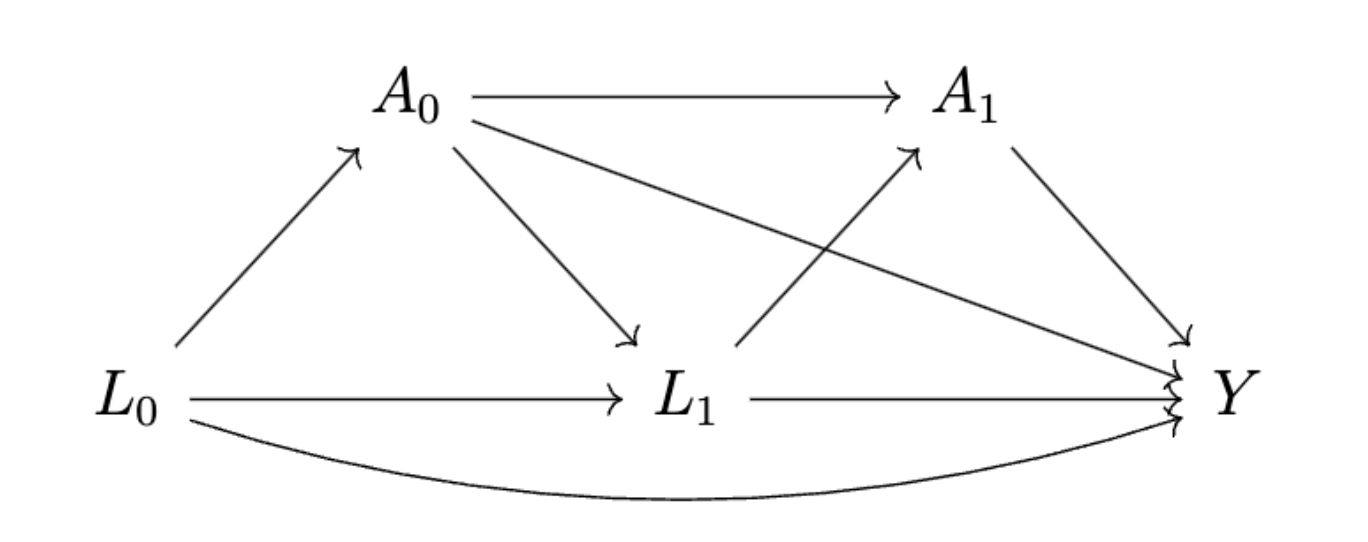
\includegraphics{img/dag.png}

Could have many more time points, high dimensional variables, competing
events, censoring nodes etc.
\end{frame}

\begin{frame}{Intervention notation}
\protect\hypertarget{intervention-notation}{}
\begin{itemize}
\item
  \(H_t\): history of data measured up to right before \(A_t\)

  \begin{itemize}
  \tightlist
  \item
    \(H_0=L_0\)
  \item
    \(H_1 = (L_0, A_0, L_1)\)
  \end{itemize}
\item
  Conceptualize treatment policies in terms of hypothetical
  interventions on nodes of the DAG
\item
  Interventions: consider a user-given function
  \(\mathsf{d}_0(a_0, h_0, \epsilon_0)\) which maps a treatment value
  \(a_0\), a history \(h_0\), and a possible randomizer \(\epsilon_0\)
  into a potential treatment value
\end{itemize}
\end{frame}

\begin{frame}{Intervention notation}
\protect\hypertarget{intervention-notation-1}{}
\begin{itemize}
\tightlist
\item
  Intervention \(\mathsf{d}_0(a_0, h_0, \epsilon_0)\) defined by
  removing node \(A_0\) from the DAG and replacing it with
  \(A_0^\mathsf{d}= \mathsf{d}_0(A_0, H_0, \epsilon_0)\)

  \begin{itemize}
  \tightlist
  \item
    This assignment generates counterfactual data:

    \begin{itemize}
    \tightlist
    \item
      \(H_1(A_0^\mathsf{d})\): counterfactual history
    \item
      \(A_1(A_0^\mathsf{d})\): natural value of treatment, i.e.~the
      value that treatment would have taken if the intervention is
      performed at time \(t=0\) but discontinued thereafter
    \end{itemize}
  \end{itemize}
\item
  At time \(t=1\), the intervention is defined by a function
  \(\mathsf{d}_1(a_1, h_1, \epsilon_1)\)

  \begin{itemize}
  \tightlist
  \item
    However, at \(t=1\) (and all subsequent times if there are more than
    two time points), the function must be applied to both the natural
    value of treatment \emph{and} the counterfactual history
  \item
    Remove node \(A_1\) from the DAG and replacing it with
    \(A_1^\mathsf{d}= \mathsf{d}_1(A_1(A_0^\mathsf{d}), H_1(A_0^\mathsf{d}), \epsilon_1)\)
  \end{itemize}
\item
  We refer to these longitudinal interventions, and the subsequent
  methods to identify and estimate effects under such interventions, as
  LMTPs
\end{itemize}
\end{frame}

\hypertarget{review-of-static-and-dynamic-interventions}{%
\section{Review of static and dynamic
interventions}\label{review-of-static-and-dynamic-interventions}}

\begin{frame}{Static interventions}
\protect\hypertarget{static-interventions}{}
\begin{itemize}
\item
  All units receive the same treatment

  \begin{itemize}
  \item
    For two time points, conceptualize a hypothetical world in which all
    units are treated at both time points (\(\mathsf{d}_t = 1\) for
    \(t \in \{0, 1\}\))
  \item
    Contrast to a hypothetical world in which no units are treated at
    either time point (\(\mathsf{d}_t = 0\) for \(t \in \{0, 1\})\)
  \item
    Gives rise to the well-known Average Treatment Effect (ATE)
  \end{itemize}
\end{itemize}
\end{frame}

\begin{frame}{Static intervention examples}
\protect\hypertarget{static-intervention-examples}{}
\begin{itemize}
\tightlist
\item
  Hypothetical intervening on a population to:

  \begin{itemize}
  \tightlist
  \item
    treat everyone with a drug versus treat no one with a drug
  \item
    enforce 30 minutes of moderate exercise for all individuals, every
    day
  \item
    give all individuals an exact level of antibodies for a certain
    disease
  \item
    setting a certain level of air quality each day, for all
    geographical areas of interest
  \end{itemize}
\end{itemize}
\end{frame}

\begin{frame}{Dynamic interventions}
\protect\hypertarget{dynamic-interventions}{}
\begin{itemize}
\tightlist
\item
  Intervention depends only on a study unit's past covariates

  \begin{itemize}
  \tightlist
  \item
    Can include past treatment
  \end{itemize}
\item
  Often used in observational studies when study units need to meet an
  indication of interest for a treatment or policy to reasonably begin,
  e.g.

  \begin{itemize}
  \tightlist
  \item
    severity of illness indicator
  \item
    socioeconomic threshold to begin a policy
  \end{itemize}
\end{itemize}
\end{frame}

\begin{frame}{Dynamic interventions}
\protect\hypertarget{dynamic-interventions-1}{}
One of the first uses of dynamic interventions was in the context of
HIV, where investigators were interested in the effect of initiating
antiretroviral therapy for a person with HIV if their CD4 count falls
below a threshold, e.g.~200 cells/\(\mu\)l (Hernán et al. 2006)

\begin{align*}
\mathsf{d}_t(h_t)=\begin{cases}
      1 &\text{ if } l_t^*<200 \text{ for all } s \ge t\\
      0&\text{ otherwise,}
\end{cases}
\end{align*}

where \(L_t^*\) is a variable in \(H_t\) that denotes CD4 T-cell count
\end{frame}

\begin{frame}{Dynamic intervention examples}
\protect\hypertarget{dynamic-intervention-examples}{}
Another example is studying the effect of initiating a corticosteroids
regimen for COVID-19 patients (Hoffman et al. 2022)

We estimated mortality under a hypothetical policy where corticosteroids
are administered for six days if and when a COVID-19 patient first meets
a severity of illness criteria (i.e.~low levels of blood oxygen)

\begin{align}
\mathsf{d}_t(h_t)=\begin{cases}
      1 &\text{ if } l_s^*=1 \text{ for any } s\in\{t-5,\ldots, t\}\\
      0&\text{ otherwise,}
\end{cases}
\end{align}

where \(L_t^*\) is a variable in \(H_s\) that denotes the first instance
of low levels of blood oxygen.
\end{frame}

\begin{frame}{Dynamic intervention examples}
\protect\hypertarget{dynamic-intervention-examples-1}{}
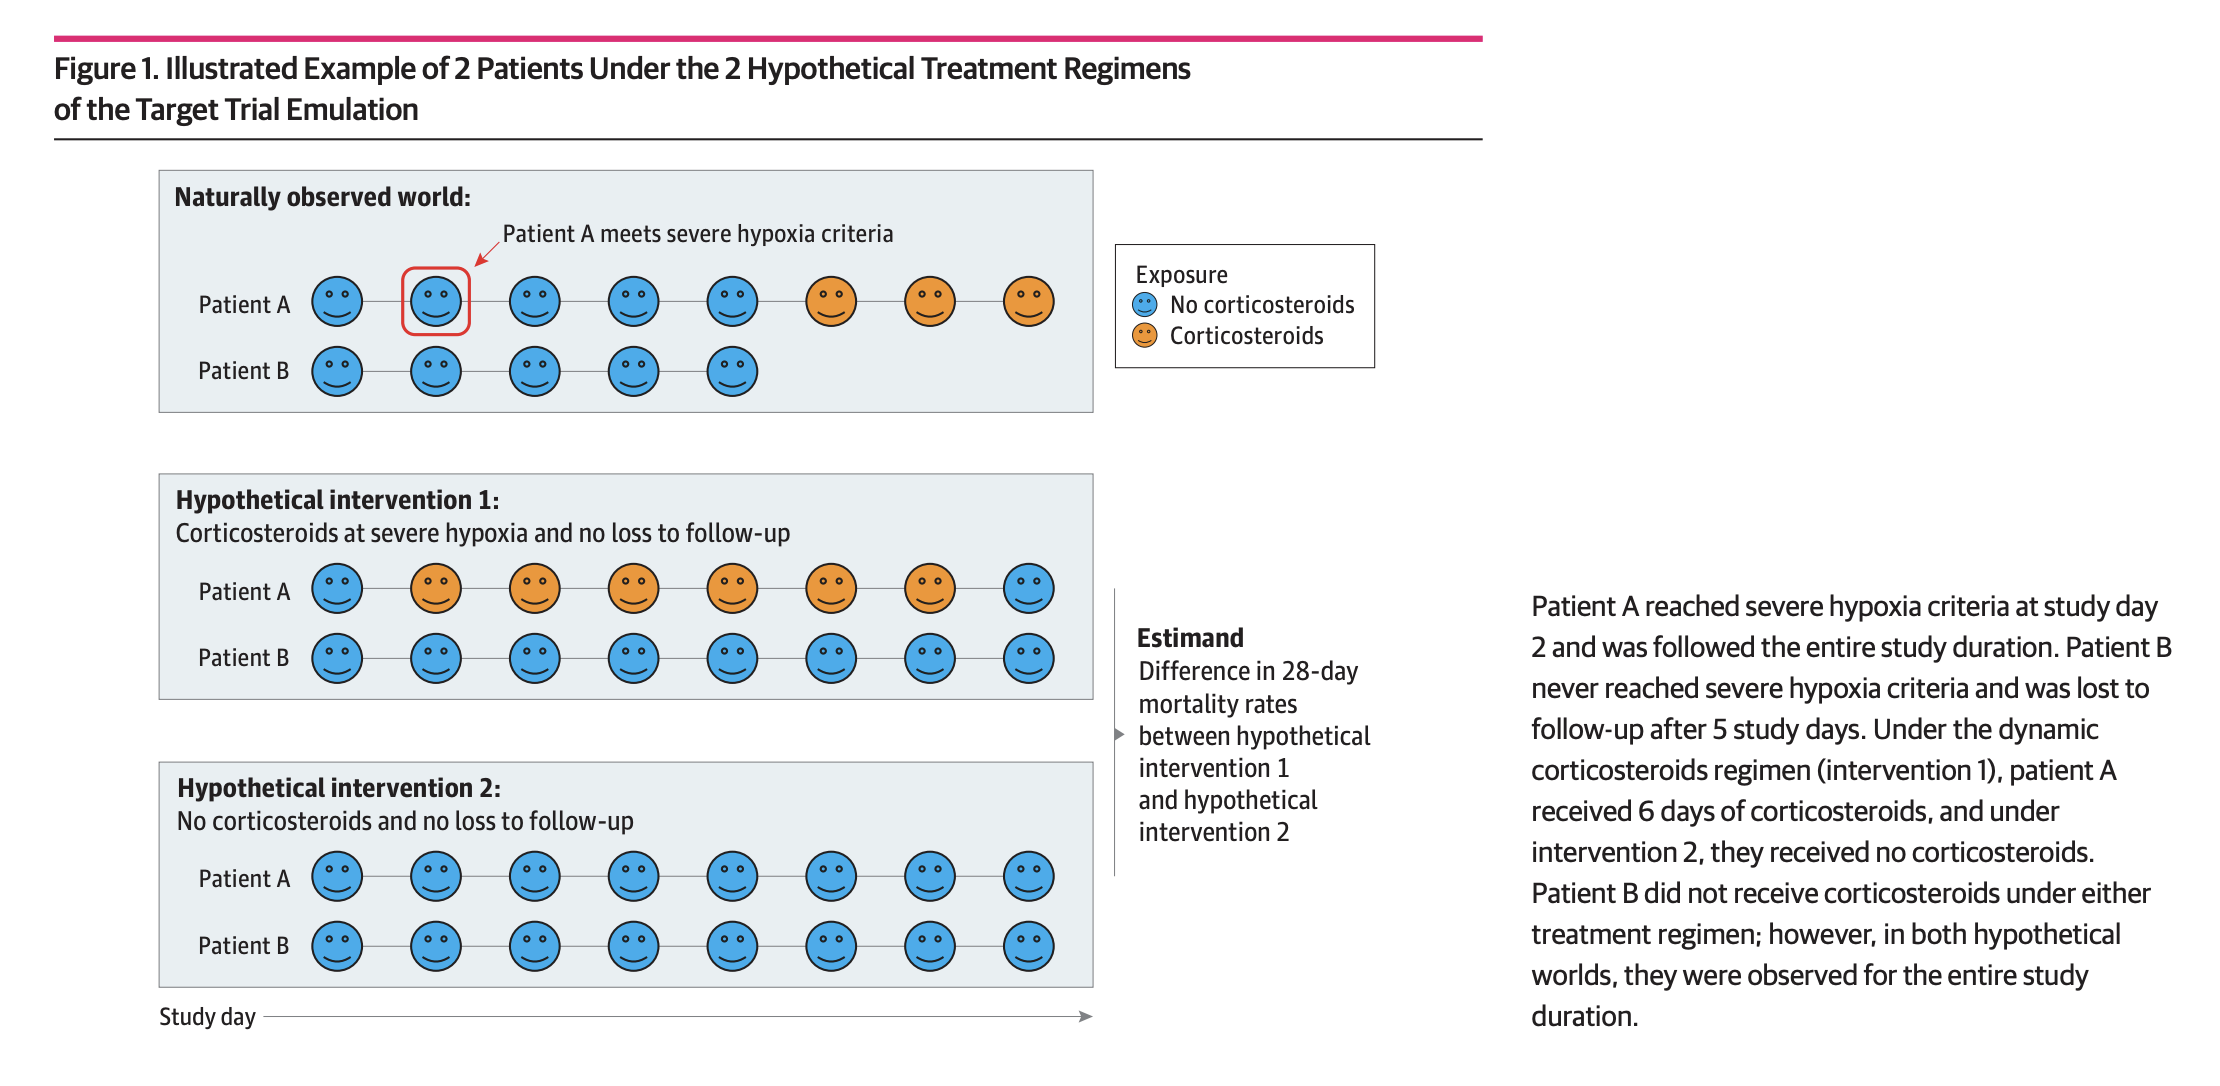
\includegraphics{img/jama_dynamic.png}
\end{frame}

\hypertarget{modified-treatment-policies}{%
\section{Modified Treatment
Policies}\label{modified-treatment-policies}}

\begin{frame}{Modified Treatment Policy}
\protect\hypertarget{modified-treatment-policy}{}
\begin{itemize}
\item
  While static and dynamic interventions are considered
  \textbf{deterministic}, MTPs are part of more general class of
  \textbf{stochastic} interventions
\item
  Intervention function \(\mathsf{d}_t(a_t, h_t, \epsilon_t)\)
  non-trivially depends on the natural value of treatment \(a_t\), and
  perhaps on \(h_t\) and/or \(\epsilon_t\)
\item
  Various types of MTPs have been proposed over the years (sometimes
  called ``interventions which depend on the natural value of
  treatment'')
\end{itemize}
\end{frame}

\begin{frame}{MTP examples: threshold functions}
\protect\hypertarget{mtp-examples-threshold-functions}{}
\textbf{Threshold function:} all natural exposure values which fall
outside of a certain boundary are intervened upon to meet a constant
value

\begin{itemize}
\item
  Could be used to assess the effect of lifestyle interventions, for
  example, intervening on individuals' average number of drinks per week
  and estimating the risk of coronary heart disease (Taubman et al.
  2009)
\item
  If we categorize drinks per week as 1 = ``none,'' 2 = ``1-5,'' 3 =
  ``6-10,'' 4 = ``11-15,'' and 5 = ``\textgreater25'', and we intervene
  to lower all individuals in the highest two drinks-per-week categories
  to ``6-10,'' we can consider that intervention in notation as,
\end{itemize}

\begin{align*}
\mathsf{d}_t(a_t)=\begin{cases}
      a_t & \text{ if } a_t < 4\\
      3 & \text{ otherwise. }
    \end{cases}
\end{align*}
\end{frame}

\begin{frame}{MTP examples: stochastic policy}
\protect\hypertarget{mtp-examples-stochastic-policy}{}
\begin{itemize}
\item
  Another example of an MTP: a hypothetical policy in which half of all
  current smokers quit smoking forever (Robins, Hernán, and Siebert
  2004)

  \begin{itemize}
  \item
    Motivated by the infeasibility of studying a world in which all
    current smokers quit smoking forever, since genetics, environment,
    and many other factors will always create some portion of current
    smokers who will never quit
  \item
    Letting \(A_t\) denote a random variable denoting smoking and
    \(\epsilon_t\) a random draw from a uniform distribution in
    \((0,1)\),
  \end{itemize}
\end{itemize}

\begin{align*}
\mathsf{d}_t(a_t,\epsilon_t)=\begin{cases}
      0 & \text{ if } \epsilon_t<0.5 \text{ and } a_t=1\\
      a_t & \text{ otherwise, }
    \end{cases}
\end{align*}
\end{frame}

\begin{frame}{MTP examples: shift functions}
\protect\hypertarget{mtp-examples-shift-functions}{}
\textbf{Shift functions} assign treatment by modifying the natural value
of the exposure by some constant \(\delta\)

\begin{itemize}
\tightlist
\item
  This intervention can be additive onto the exposure value, such as
  estimating the effect of a hypothetical intervention to reduce lung
  cancer resection surgeries lasting longer than 60 minutes by 15
  minutes (Haneuse and Rotnitzky 2013)
\end{itemize}

\begin{align*}
\mathsf{d}_t(a_t)=\begin{cases}
      a_t & \text{ if } a_t \leq 60 \\
      a_t - 15 & \text{ otherwise. }
    \end{cases}
\end{align*}
\end{frame}

\begin{frame}{MTP examples: shift functions}
\protect\hypertarget{mtp-examples-shift-functions-1}{}
\begin{itemize}
\tightlist
\item
  A shift function can also change the exposure on a multiplicative
  scale

  \begin{itemize}
  \tightlist
  \item
    For example, studying the effect of an intervention which doubles
    the number of street lights for roads with less than 10 lights per
    mile on nighttime automobile accidents
  \end{itemize}
\end{itemize}

\begin{align*}
\mathsf{d}_t(a_t)=\begin{cases}
      a_t & \text{ if } a_t \ge 10 \\
      2a_t & \text{ otherwise. }
    \end{cases}
    \end{align*}
\end{frame}

\hypertarget{causal-estimand}{%
\section{Causal estimand}\label{causal-estimand}}

\begin{frame}{Causal estimand}
\protect\hypertarget{causal-estimand-1}{}
\begin{itemize}
\item
  Once an intervention is specified, the counterfactual outcomes of
  observations under a specific \(\mathsf{d}\) are denoted as
  \(Y(\bar{A}_\tau^\mathsf{d})\), where \(\bar{A}\) indicates the
  history of measurements of \(A\) for all time points,
  i.e.~\(\bar A = (A_1, \ldots, A_\tau)\)
\item
  Causal effects are defined as a distribution of contrasts of
  \(Y(\bar{A}_\tau^\mathsf{d})\) under different interventions,
  \(\mathsf{d}'\) and \(\mathsf{d}^\star\)
\item
  In this tutorial, we focus on
  \(\mathsf{E}[Y(\bar{A}_\tau^{\mathsf{d}'}) - Y(\bar{A}_\tau^{\mathsf{d}^ {\star}})]\)
  as our causal estimand of interest

  \begin{itemize}
  \tightlist
  \item
    The functions \(\mathsf{d}'\) and \(\mathsf{d}^\star\) may be any
    type of intervention, including ``no intervention''
  \end{itemize}
\end{itemize}
\end{frame}

\hypertarget{identification}{%
\section{Identification}\label{identification}}

\begin{frame}{Identification}
\protect\hypertarget{identification-1}{}
\begin{itemize}
\item
  Now, we need to write our counterfactual expectation
  \(\mathsf{E}[Y(\bar{A}_\tau^{\mathsf{d}'})]\) as a formula that
  depends only on the observed data distribution---i.e., an identifying
  formula
\item
  This requires assumptions, some of which are untestable with the data
  available

  \begin{itemize}
  \tightlist
  \item
    The mathematically rigorous form of the assumptions is given
    elsewhere (Richardson and Robins 2013) (Díaz et al. 2021), but we
    state them in the tutorial in simple terms
  \end{itemize}
\end{itemize}
\end{frame}

\begin{frame}{Identification assumptions}
\protect\hypertarget{identification-assumptions}{}
\begin{block}{Positivity}
\protect\hypertarget{positivity}{}
\begin{itemize}
\tightlist
\item
  If it is possible to find an observation with history \(h_t\) with an
  exposure of \(a_t\), then it is also possible to find an observation
  with history \(h_t\) with an exposure \(\d(a_t, h_t, \epsilon_t)\)
\end{itemize}
\end{block}

\begin{block}{Strong sequential randomization}
\protect\hypertarget{strong-sequential-randomization}{}
\begin{itemize}
\item
  All common causes of the intervention variable \(A_t\) and
  \((U_{L,t+1}, U_{A,t+1})\) are measured and recorded in \(H_t\).

  \begin{itemize}
  \tightlist
  \item
    Generally satisfied if \(H_t\) contains all common causes of \(A_t\)
    and \((L_{t+1}, A_{t+1}, \ldots, L_\tau, A_\tau,\allowbreak Y)\),
    where \(\tau\) is the last time point in the study
  \end{itemize}
\end{itemize}
\end{block}

\begin{block}{Weak sequential randomization}
\protect\hypertarget{weak-sequential-randomization}{}
\begin{itemize}
\tightlist
\item
  All common causes of the intervention variable \(A_t\) and
  \((U_{L,t+1})\) are measured and recorded in \(H_t\)
\end{itemize}
\end{block}
\end{frame}

\begin{frame}{Identification assumptions}
\protect\hypertarget{identification-assumptions-1}{}
\begin{itemize}
\item
  While static and dynamic interventions require the weak version of
  sequential randomization, LMTPs require the strong version
\item
  Violations to the positivity assumption can be \textbf{structural} or
  \textbf{practical}

  \begin{itemize}
  \item
    \textbf{Structural}: certain characteristics of an individual or
    unit which will never yield receipt of the treatment assignment
    under the intervention. This violation will not improve even with an
    infinite sample size.
  \item
    \textbf{Practical}: Due to random chance or small datasets, there
    are certain covariate combinations with zero or near-zero predicted
    probabilities of treatment.
  \end{itemize}
\end{itemize}
\end{frame}

\begin{frame}{Positivity, cont.}
\protect\hypertarget{positivity-cont.}{}
\begin{itemize}
\item
  Positivity violations increase the finite bias and variance of
  estimates and severely threaten the validity of casual inference
  analyses when not addressed
\item
  For time-varying treatments, positivity must be maintained at each
  time point
\item
  By design, non-static interventions (e.g.~dynamic treatment rules,
  MTPs) may help define estimands with plausible positivity, since the
  function \(\mathsf{d}\) can be modified to affect the exposure of only
  observations which are not subject to positivity violations
\end{itemize}
\end{frame}

\begin{frame}{Example of redefining an estimand}
\protect\hypertarget{example-of-redefining-an-estimand}{}
\begin{itemize}
\item
  Think of a world in which a continuous exposure is observed at some
  fixed value higher or lower than it was factually observed for every
  unit in the study

  \begin{itemize}
  \tightlist
  \item
    EX: surgery times were 15 minutes shorter for all lung resection
    biopsies
  \end{itemize}
\item
  This hypothetical intervention is destined for structural positivity
  violations, because at the lowest end of the observed exposure range,
  there will by definition be no support for the intervened exposure
  level \(\mathsf{d}(a_t)\) (much less conditional on the observation's
  history \(h_t\))
\item
  This can be avoided by constraining the range of \(a_t\) affected by
  the hypothetical intervention, so that no \(\mathsf{d}(a_t)\) values
  are produced outside the observed range of \(A\)

  \begin{itemize}
  \tightlist
  \item
    Could modify intervention to accommodate any other remaining
    structural or practical positivity violations
  \end{itemize}
\end{itemize}
\end{frame}

\hypertarget{identification-formula}{%
\section{Identification formula}\label{identification-formula}}

\begin{frame}{Identification formula}
\protect\hypertarget{identification-formula-1}{}
\begin{itemize}
\item
  Under positivity and strong (or weak) sequential randomization
  assumptions, the estimand is identified by the generalized g-formula
\item
  A re-expression of this generalized g-formula involves recursively
  defining the expected outcome under the intervention conditional on
  the observation's observed exposure and history

  \begin{itemize}
  \tightlist
  \item
    beginning at the final time point, and proceeding until the earliest
    time point
  \end{itemize}
\end{itemize}
\end{frame}

\begin{frame}{Identification formula}
\protect\hypertarget{identification-formula-2}{}
\begin{enumerate}

\item Start with the conditional expectation of the outcome $Y$ given $A_1=a_1$ and $H_1=h_1$. Let this function be denoted $Q_1(a_1, h_1)$
\item Evaluate the above conditional 
  expectation of $Y$ if $A_1$ were changed to $A^\mathsf{d}_1$, which results in 
  a pseudo outcome $\tilde Y_1=Q_1(A^\mathsf{d}_1, H_1)$
\item Let the true expectation of $\tilde Y_1$ conditional on
  $A_0=a_0$ and $H_0=h_0$ be denoted $Q_0(a_0, h_0)$
\item Evaluate the above
  expectation of $\tilde Y_1$ if $A_0$ were changed to $A^\mathsf{d}_0$, which results in
  $\tilde Y_0=Q_0(A^\mathsf{d}_0, H_0)$
\item Under the identifying assumptions, we have
  $\mathsf{E}[Y(\bar{A}_\tau^\mathsf{d})]=\mathsf{E}[\tilde Y_0]$
  
\end{enumerate}
\end{frame}

\hypertarget{estimation}{%
\section{Estimation}\label{estimation}}

\begin{frame}{References}
\protect\hypertarget{references}{}
For more information:

\hypertarget{refs}{}
\begin{CSLReferences}{1}{0}
\leavevmode\vadjust pre{\hypertarget{ref-diaz_nonparametric_2021}{}}%
Díaz, Iván, Nicholas Williams, Katherine L. Hoffman, and Edward J.
Schenck. 2021. {``Nonparametric {Causal} {Effects} {Based} on
{Longitudinal} {Modified} {Treatment} {Policies}.''} \emph{Journal of
the American Statistical Association}, September, 1--16.
\url{https://doi.org/10.1080/01621459.2021.1955691}.

\leavevmode\vadjust pre{\hypertarget{ref-haneuse2013estimation}{}}%
Haneuse, Sebastian, and Andrea Rotnitzky. 2013. {``Estimation of the
Effect of Interventions That Modify the Received Treatment.''}
\emph{Statistics in Medicine} 32 (30): 5260--77.

\leavevmode\vadjust pre{\hypertarget{ref-hernan2006comparison}{}}%
Hernán, Miguel A, Emilie Lanoy, Dominique Costagliola, and James M
Robins. 2006. {``Comparison of Dynamic Treatment Regimes via Inverse
Probability Weighting.''} \emph{Basic \& Clinical Pharmacology \&
Toxicology} 98 (3): 237--42.

\leavevmode\vadjust pre{\hypertarget{ref-hoffman2022comparison}{}}%
Hoffman, Katherine L, Edward J Schenck, Michael J Satlin, William
Whalen, Di Pan, Nicholas Williams, and Iván Dı́az. 2022. {``Comparison of
a Target Trial Emulation Framework Vs Cox Regression to Estimate the
Association of Corticosteroids with COVID-19 Mortality.''} \emph{JAMA
Network Open} 5 (10): e2234425--25.

\leavevmode\vadjust pre{\hypertarget{ref-richardson2013single}{}}%
Richardson, Thomas S, and James M Robins. 2013. {``Single World
Intervention Graphs (SWIGs): A Unification of the Counterfactual and
Graphical Approaches to Causality.''} \emph{Center for the Statistics
and the Social Sciences, University of Washington Series. Working Paper}
128 (30): 65--78.

\leavevmode\vadjust pre{\hypertarget{ref-robins2004effects}{}}%
Robins, James M, Miguel A Hernán, and Uwe Siebert. 2004. {``Effects of
Multiple Interventions.''} \emph{Comparative Quantification of Health
Risks: Global and Regional Burden of Disease Attributable to Selected
Major Risk Factors} 1: 2191--2230.

\leavevmode\vadjust pre{\hypertarget{ref-taubman2009intervening}{}}%
Taubman, Sarah L, James M Robins, Murray A Mittleman, and Miguel A
Hernán. 2009. {``Intervening on Risk Factors for Coronary Heart Disease:
An Application of the Parametric g-Formula.''} \emph{International
Journal of Epidemiology} 38 (6): 1599--1611.

\end{CSLReferences}
\end{frame}



\end{document}
